%% LaTeX2e class for seminar theses
%% seminar.tex
%% 
%% Karlsruhe Institute of Technology
%% Institute for Program Structures and Data Organization
%% Chair for Software Design and Quality (SDQ)
%%
%% Dr.-Ing. Erik Burger
%% burger@kit.edu
%%
%% Version 1.0.3, 2020-06-26

%% Available page modes: oneside, twoside
%% Available languages: english, ngerman
%% Available modes: draft, final (see README)
\documentclass[twoside, english]{sdqseminar}

%% ---------------------------------
%% | Information about the thesis  |
%% ---------------------------------

%% Name of the author
\author{Tim Engbrocks}

%% Title (and possibly subtitle) of the thesis
\title{Optimization Approaches for Self-Adaptive Systems}

%% Type of the thesis 
% \thesistype{Seminar Thesis}

%% Change the institute here, ``IPD'' is default
% \myinstitute{Institute for \dots}

%% The advisors are PhD Students or Postdocs
\advisor{Dipl.-Inform. Martina Rapp}

\settitle

%% --------------------------------
%% | Settings for word separation |
%% --------------------------------

%% Describe separation hints here.
%% For more details, see 
%% http://en.wikibooks.org/wiki/LaTeX/Text_Formatting#Hyphenation
\hyphenation{
% me-ta-mo-del
}

%% --------------------------------
%% | Bibliography                 |
%% --------------------------------

%% Use biber instead of BibTeX, see README
\usepackage[citestyle=numeric,style=numeric,backend=biber]{biblatex}
\addbibresource{seminar.bib}

%% ====================================
%% ====================================
%% ||                                ||
%% || Beginning of the main document ||
%% ||                                ||
%% ====================================
%% ====================================
\begin{document}

%% Set PDF metadata
\setpdf

%% Set the title
\maketitle

%% ----------------
%% |   Abstract   |
%% ----------------
 
%% The text is included from the following files:
%% - sections/abstract

% NOTE: Planned pages -> minimum of 15 content pages
% Chapter           Planned Current Missing
% Introduction:     2       2       0
% Classification:   5       4       1
% Proposal:         5       4.5     0.5
% Existing:         2       0.5     1.5
% Conclusion:       1       0       1
% Total:            15      8.5     4

% CURRENT TODO:
% - Abstract fehlt noch
% - Was trägt self-* zum Proposal bei?
% 	- Evtl Paper nochmal lesen
% - klarer machen das der 5w+1h teil in classification nicht von mir stammt
% 	- manche punkte könnten ausführlicher sein
% - classification: ausführlicher wie diese drei dimensions optimized werden können
% - proposal: übergang mape mapping zu dimensions erklärung
% 	- klarstellung dass es ein proposal ist
% - Erklärung dimensions: Text bei Approach
% - Maybe short summary sentence am ende von proposal vor den tables
	
% . ML usage paper: Bezug auf die dort proposed classification?

- Introduction ist gut

% ABSTRACT WIRD ALS LETZTES GESCHRIEBEN!

% \begin{abstract}
%     Content of the abstract: \begin{itemize}
%         \item Motivating \acrlong{sas}[s] and their need for optimization.
%         \item Motivating the need for a classification of \acrlong{oa}es for \acrlong{sas}[s].
%         \item The scope and goal of this paper.
%     \end{itemize}
% \end{abstract}

\begin{abstract}
    \textbf{Abstract} \ \ The complexity of modern software systems is constantly growing.
    This requires new ways to be found to better manage large scale software systems.
    \acrlong{sas}[s] which autonomously manage themselves using well-defined rules
    are a solution to this problem.
    Even tough these systems are able to adapt themselves,
    they struggle with unpredicted changes in their context.
    This can be solved by using \acrlong{oa}[es] for \acrlong{sas}[s] which can optimize these systems.
    There are already many \acrlong{oa}[es], but no way to classify them.
    This paper proposes a classification for \acrlong{oa}[es] for \acrlong{sas}[s].
\end{abstract}
\section{Introduction}
\label{ch:Introduction}

\begin{figure*}[hbt!]
    \centering
    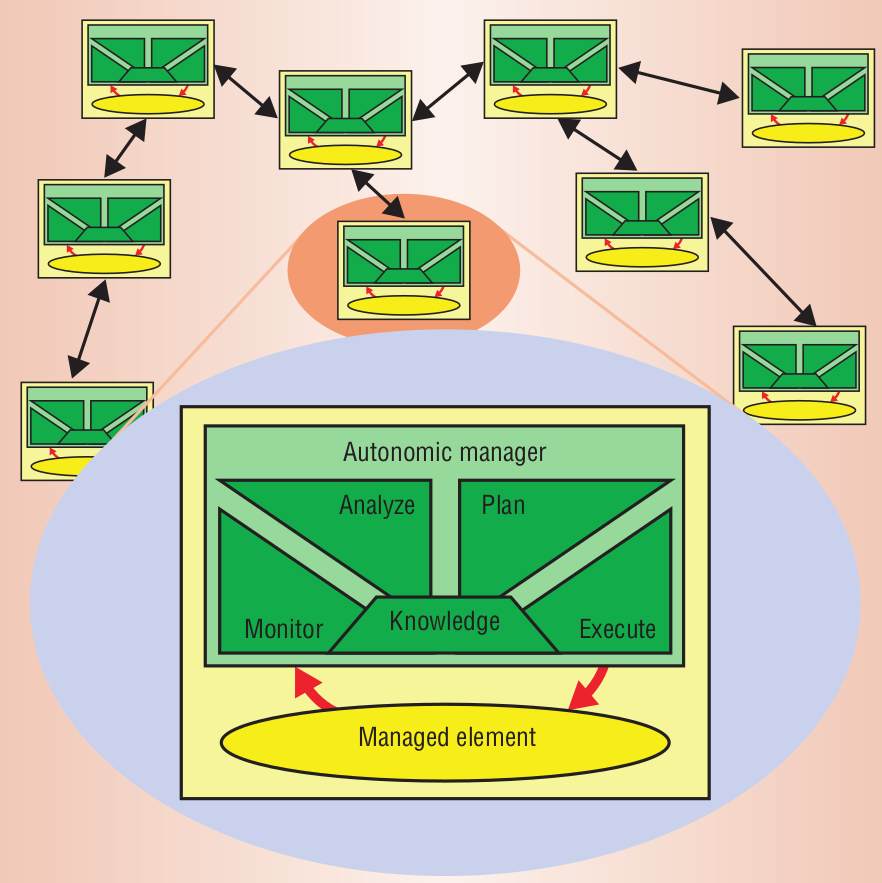
\includegraphics[width=0.6\textwidth]{images/MAPEK.png}
    \caption{The \acrshort{mapek} (Monitor-Analyze-Plan-Execute with Knowledge) feedback loop by Kephart and Chess, 2003 \cite*{VisionOfAutonomicComputing}}
    \label{fig:MAPEK}
\end{figure*}

The complexity of modern software systems is constantly growing.
Most of this growth in complexity stems from the
"need to integrate several heterogeneous environments into corporate-wide computing systems,
and to extend that beyond company boundaries into the Internet" (Kephart and Chess, 2003 \cite*{VisionOfAutonomicComputing}).
This has reached a state where the
"complexity appears to be approaching the limits of human capability" (Kephart and Chess, 2003 \cite*{VisionOfAutonomicComputing}).
In combination with the uncertainty about a software systems future operations and environment,
that the developers of such complex systems face, it becomes uneconomical to purely operate such a system by human operators.

\noindent From this the need for software systems which can autonomously manage themselves arises.
In order to achieve this task of autonomous self-management, the system has to be able to:
\begin{itemize}[nosep]
    \item detect faults and changes in its environment,
    \item analyze them,
    \item decide how to react to them
    \item and make changes to itself.
\end{itemize}

\newpage
\noindent To model these abilities Kephart and Chess developed
the \acrfull{mapek} feedback loop \cite*{VisionOfAutonomicComputing} shown in Figure \ref{fig:MAPEK}.

\noindent First the system has to \textit{monitor} itself and its environment.
The data, gathered by the monitoring step, has to be \textit{analyzed} to detect changes and faults.
If the analyzing step detects, that an adaptation is necessary,
the system has to \textit{plan} how to perform the necessary changes.
After the changes have been planned, they need to be \textit{executed}.
All of this happens with \textit{knowledge} of the environment and the system.

\noindent Software systems that can autonomously manage themselves are called \acrfull{sas}[s]
because of their ability to adapt themselves.

\noindent To better understand \acrshort{sas}, let us take a look at a commonly used example.
Imaging you are the system administrator of a large scale online store.
This store has four parameters: site traffic, number of purchases, number of active server instances and the number of served advertisements.
During your day to day operations you encounter a common type of task:
Update some system parameter X based on some metric Y.
To make your job easier, you decide to use a \acrshort{sas} for these tasks
and come up with the following generalized adaptation rule:
If metric Y crosses threshold Z, update the system parameter X.

\noindent In this case the usage of a \acrshort{sas} was beneficial because it could easily
automate a general set of tasks.
A human operator might have been able to perform these tasks on his own,
if the number of system parameters was sufficiently small.
But the \acrshort{sas} is better at handling large numbers of system parameters.


\noindent While \acrshort{sas} are better at handling more complex systems,
human operators are better at handling uncertainty.
This has two reasons. 
Firstly, the adaptation rules and policies used by \acrshort{sas} are statically created at design time.
Secondly, \acrshort{sas} can adapt the software that they are managing but they can not change their adaptation process.
Over time this leads to an increasing divergence between the expected results of adaptations and the actual results,
when the environment changes in ways that were not predicted by developers during the design time of the system.

\noindent This can be illustrated by the previous example.
Imagine that the \acrshort{sas} has been in operation for some and you collected data on the systems performance.
You notice that the \acrshort{sas} changes some system parameters too aggressively,
because it performs an adaptation as soon as a metrics threshold has been violated.
As a human operator you would have waited some time to see how the metric develops before performing an adaptation
which would result in a smoother operation.
The \acrshort{sas} can not handle this type of uncertainty and only reacted to the current state of its environment.

\noindent Optimizations are necessary to improve the performance and effectiveness of \acrshort{sas} in situations like these.
There are already many approaches on how to optimize \acrshort{sas}.
Some of them focus on updating adaptation rules and policies during the systems runtime.
Others dynamically change at which level of the system adaptations are performed.
Generally most optimizations target static components of \acrshort{sas}.
These components can be improved by making them more dynamic, 
which is often achieved by applying modern learning methods.

\noindent The previous example could benefit from such optimizations by dynamically updating adaptation rules
to better reflect the systems changing environment.

\noindent While there are already many \acrfull{oa}[es] for \acrshort{sas},
there is no classification for them.
Because of this, the existing \acrshort{oa} can not be easily compared
and it is difficult to identify areas which require further research.
This paper aims to provide such a classification for \acrlong{oa}[es] for \acrlong{sas}[s].

\noindent To derive a classification for \acrshort{oa} for \acrshort{sas},
chapter \ref{ch:SASClassification} will first explain how \acrshort{sas} are classified
using three different approaches.
Based on these approaches, a classification for \acrshort{oa} for \acrshort{sas} will be derived
and proposed in chapter \ref{ch:Proposal}.
In chapter \ref{ch:Existing} the proposed classification will be applied to some existing \acrshort{oa}.
Lastly, chapter \ref{ch:Conclusion} will finish with a conclusion and recommendations for future research directions.

\newpage
\section{Classification of Self-Adaptive Systems}
\label{ch:SASClassification}

There are different approaches on how to classify and describe \acrshort{sas} which all focus on different usages.
The three approaches that will be highlighted by this section are:
\begin{itemize}[nosep]
    \item FORMS \cite*{FORMS}
    \item Berns' and Ghosh's definition of self-* properties \cite*{DissectingSelfProperties}
    \item Krupitzer's et al. taxonomy for \acrshort{sas} \cite*{SurveyOnEngineeringApproaches}
\end{itemize} 
These approaches contain ideas that will be used to construct the classification for
\acrshort{oa} for \acrshort{sas} in the next chapter.

\begin{figure*}[b!]
    \centering
    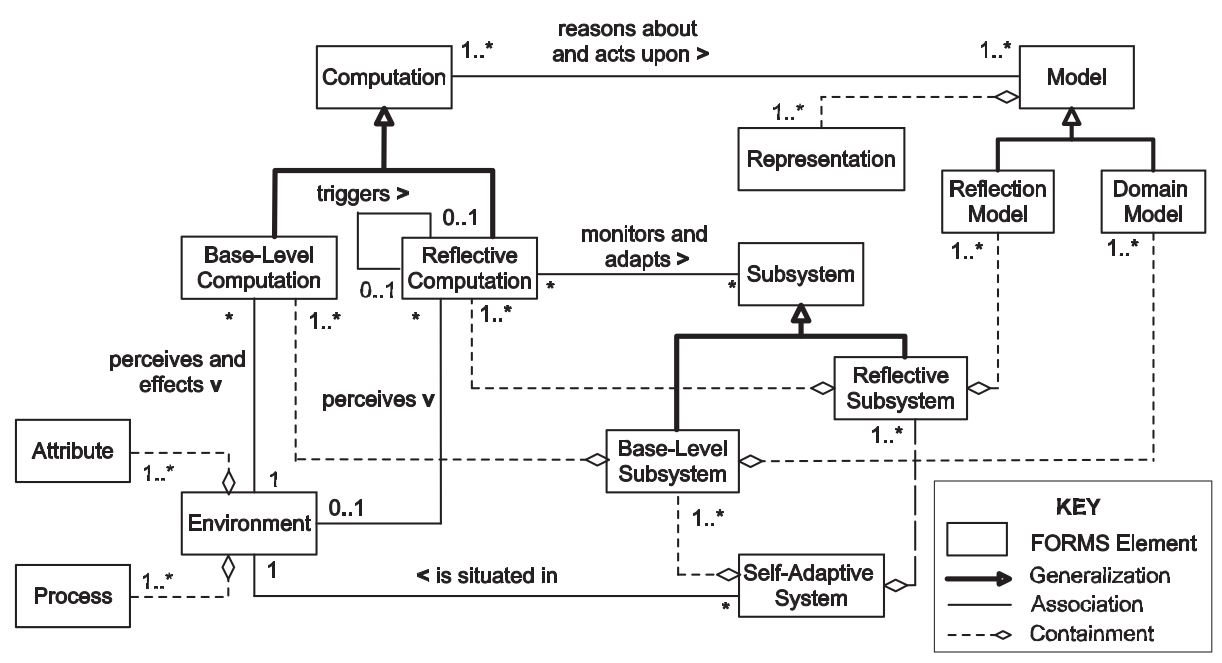
\includegraphics[width=\textwidth]{images/FORMS.png}
    \caption{FORMS primitives \cite*{FORMS}}
    \label{fig:FORMS}
\end{figure*}

\noindent With FORMS Weyns et al. propose a formal reference model for describing \acrshort{sas} \cite{FORMS}.
The goal of FORMS is to provide a well defined basis for talking and reasoning about \acrshort{sas}.
This is achieved by constructing \acrshort{sas} from a set of primitives which are defined in Z notation.
Z notation is used for formal specifications and is based upon Zermelo-Fraenkel set theory.
It is mathematically well-defined and often used to describe software systems.

\noindent Figure \ref{fig:FORMS} shows all the primitives used by FORMS and their relationships.
The \acrshort{sas} is split into different layers of subsystems.
Base-level refers to subsystems on the bottom most layer of the system.
Subsystems in layers above the base-level layer are called reflective.
Reflection refers to the ability of a system to inspect and change itself.

\noindent Each subsystem consists of two parts: its computation and its model.
Base-level subsystems have domain models which contain data about the environment.
In addition to that, reflective subsystems also have a reflection model which contains data about the system itself.
While base-level subsystems can use their computation to affect the environment,
reflective subsystems can affect the subsystems in the layer below themselves.

\noindent This approach can be understood with the example of a robot that uses motorized wheels
and some sensors to observe its environment.
The motor control software used by the robot would be placed in the base-level layers.
The sensors would be placed in the base-level layer as well.
These components are responsible for observing the environment and interacting with it.
On top of the base-level layer the robot might use a reflective layer which changes how the wheels are operated
based on the current weather conditions that it observes.
The top layer of the robots software could be an automatic updater 
which automatically updates the robots software to the latest version.
For this, the updater has to examine the robots software and modify it.
In other words, the updater is a reflective component.

\noindent The concept of different layers of reflection will be useful later to distinguish
\acrshort{oa} from \acrshort{sas}.

%% self-* properties
\begin{figure*}[t!]
    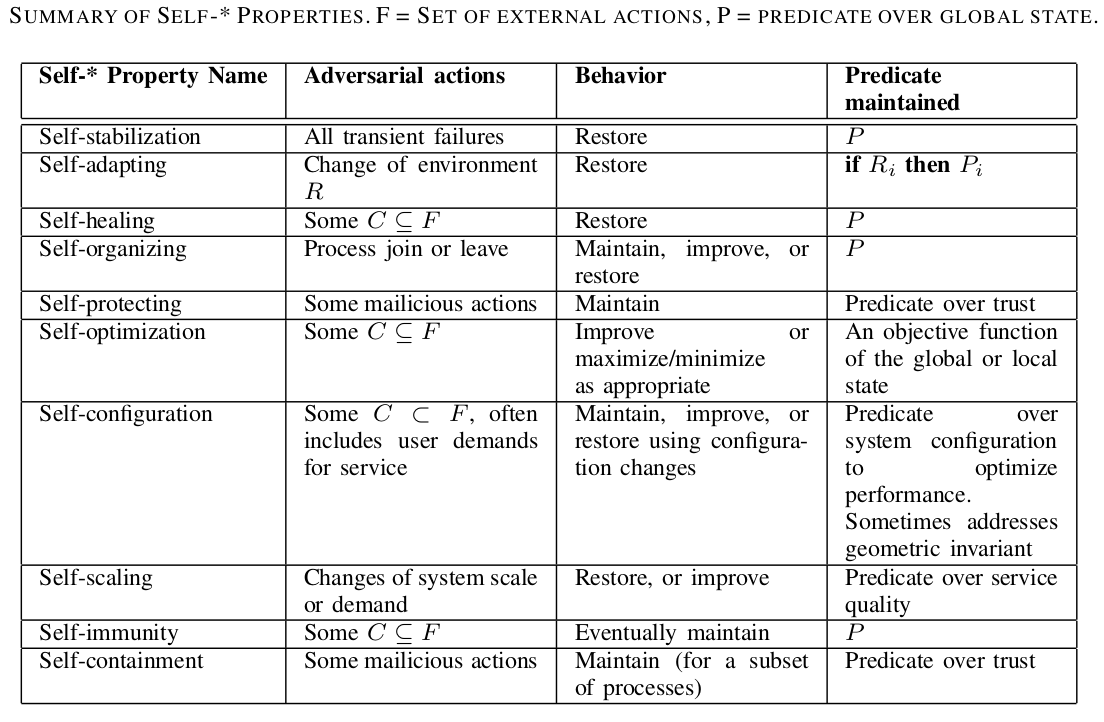
\includegraphics[width=\textwidth]{images/SelfProperties.png}
    \caption{self-* properties \cite*{DissectingSelfProperties}}
    \label{fig:SelfProperties}
\end{figure*}

\noindent Although some of the first papers on \acrshort{sas}, for example, 
"The Vision of Autonomic Computing" by Kephart and Chess \cite*{VisionOfAutonomicComputing} focused on self-adaptation,
there are other aspects of software systems that can benefit from the ideas introduced by \acrshort{sas}.
Berns and Ghosh identified and described such aspects which they call self-* properties \cite*{DissectingSelfProperties}.
They found the self-* properties that are depicted in Figure \ref{fig:SelfProperties}.

\noindent Berns and Ghosh describe \acrshort{sas} in terms of their interaction with their environment
and their reaction to external actions \cite*{DissectingSelfProperties}.
External actions are actions stemming from the systems environment which affect the system directly.
Safety predicates are used to describe goals of the system.
These external actions are called malicious if the intent of the action is the violation of a safety predicate.
A system also has a configuration which is the collection of its parameters.
Using these definitions, Berns and Ghosh describe their self-* properties in the following way:

\subparagraph*{Self-stabilization}
A system has the self-stabilization property if it can get from any starting configuration
to a configuration in which its safety predicates are fulfilled and stay in such a configuration afterwards.
In other words: The system can complete its starting procedure without requiring assistance.
\subparagraph*{Self-adapting}
A system is self-adapting (or managing) if it maintains, improves or restores safety predicates
without human intervention.
This definition matches the definition proposed by Kephart and Chess \cite*{VisionOfAutonomicComputing}
of systems which can autonomously manage themselves without human intervention.
\subparagraph*{Self-healing}
A system is self-healing if an external action can only cause a temporary violation of safety predicates.
This means that a self-healing system can recover from external actions on its own.
An example would be a system which can restart itself after a power outage.
\subparagraph*{Self-organizing}
A system is self-organizing if it maintains, improves or restores safety predicates after an external
action which involves processes joining or leaving the system. The recovery time per join or leave should be sublinear.
Peer-to-peer networks can be examples for self-organizing systems.
\subparagraph*{Self-protecting}
A system is self-protecting if it maintains one chosen safety predicate even when malicious external actions occur.
Meaning that a self-protecting system guarantees that it will never violate the chosen safety predicate.
A real world example for this would be a system which guarantees that it will not disclose personal data to unauthorized users.
\subparagraph*{Self-optimization}
When a system is self-optimizing, it can maximize or minimize the value of a utility function.
A system which starts and stops services based on demand to reduce energy usage is an example for a self-optimizing system.
\subparagraph*{Self-configuration}
A system possesses the self-configuration property if it can change its configuration to restore or improve a safety predicate.
\subparagraph*{Self-scaling}
A self-scaling system can maintain or improve a system property while an external action affects its scale.
This means that a system which regulates the number of instances of one of its services based, for example, on demand is self-scaling.
\subparagraph*{Self-immunity}
A system with self-immunity can restore safety predicates after the occurrence of external actions
and return to a state where no safety predicate is violated as if the external action never happened.
\subparagraph*{Self-containment}
A system is self-containing if a malicious external action can not compromise the whole system
and the system is able to eventually return to its normal operating state.

\noindent These self-* properties are useful to:
\begin{itemize}[nosep]
    \item Communicate the abilities and goals of a system.
    \item Establish well-defined goals for the system.
\end{itemize}
They show that there are aspects besides the management of software which can benefit from the ideas of self-adaptation.
This can be used as it distinguishes \acrshort{sas} from system with other self-* properties.
The only other self-* property that will be important for the rest of this paper is the self-optimization property.

\begin{figure*}[t!]
    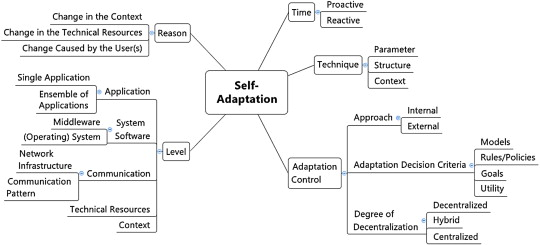
\includegraphics[width=\textwidth]{images/KrupitzerTaxonomy.jpg}
    \caption{Taxonomy for \acrshort{sas} \cite*{SurveyOnEngineeringApproaches}}
    \label{fig:KrupitzerTaxonomy}
\end{figure*}

\noindent The taxonomy for \acrshort{sas} in Figure \ref{fig:KrupitzerTaxonomy}
is based upon the 5W+1H questions by Salehie and Tahvildari, 2009 \cite*{LandscapeAndResearchChallenges}.
These questions are: Where, When, What, Why, Who and How.
Each of these questions is responsible for a different aspect of \acrshort{sas} and corresponds to a dimension of the taxonomy.

\subparagraph*{Why}
First there needs to be a reason for a \acrshort{sas} to adapt. Why an adaptation should be performed is answered by the Reason dimension.
According to the taxonomy reasons for an adaptation can be changes in either the context, a technical resource or changes caused by the user.

\subparagraph*{Where}
The question of where asks on which level of the system changes need to occur.
The different levels on which changes can occur include:
\begin{itemize}[nosep]
    \item Different levels of applications from the operating system to a user application
    \item How systems communicate with each other
    \item The technical resources that are needed by the system
    \item The context in which the system operates
\end{itemize}

\subparagraph*{When}
While the original When-Question by Salehie and Tahvildari tries to understand all temporal aspects of \acrshort{sas},
including how frequently changes should occur and if they happen continously,
the taxonomy only answers the question when changes should be performed.
For this purpose the Time dimension differentiates between systems that perform changes proactively or reactively.
Reactive changes occur after, for example, a system metric has been violated.
Proactive changes occur before a system metric can be violated.

\subparagraph*{What}
In addition to the question of where and when changes should occur, it is also important to know
what changes should occur. There are different techniques that can be used.
The Technique dimension of the taxonomy differentiates between systems that change parameters, their structure or their context.
A system that changes its structure could, for example, be a datacenter, which starts new server instances on demand.
Robots are an example for systems that change their context.
This is achieved by, for example, moving the robot around.

\subparagraph*{Who}
After answering where, when, what and why changes should be performed, 
it is necessary to select who is responsible for these changes.
According to Salehie and Tahvildari it is also important to establish if the changes can be performed fully autonomous
or if the involvement of human operators is necessary.
The taxonomy does not directly address all of these concerns but states that:
"N/A (nature of a SAS leads to an automatic type of adaptation)" \cite{SurveyOnEngineeringApproaches}.

\subparagraph*{How}
Lastly, after determining the where, when, what, why and who, there needs to be a way
to perform the required changes. This is answered by asking how the changes should be performed
and corresponds to the Adaptation Control.
The three main aspects of the Adaptation Control are the degree of decentralization, the adaptation decision criteria
and the approach taken by the system.
The degree of decentralization ranges from systems which perform adaptations through a central component (fully centralized)
to systems where each component is responsible for its own adaptation (fully decentralized).
In between these two degrees are systems that employ a hybrid approach.
The adaptation decision criteria controls how the adaptation is achieved.
Krupitzer et al. propose the following possibilities:
\begin{itemize}[nosep]
    \item Models: The \acrshort{sas} updates e.g. domain models which results in behavioral changes
    \item Rules/Policies: The \acrshort{sas} changes its behavior based on rules or policies
    \item Goals: The \acrshort{sas} changes its behavior to meet some predefined set of goals
    \item Utility: The \acrshort{sas} changes its behavior to maximize or minimize a utility function
\end{itemize}
The approach divides \acrshort{sas} into those where the adaptation logic is part of the application logic
and those with separated adaptation and application logic.

\noindent After classifying \acrshort{sas} the following question can be asked: Which parts of a \acrshort{sas} can be optimized?
To answer this we will start by looking at which parts can not be optimized or do not benefit from optimization.

\noindent The first part that can not be optimized is the environment which provides the Reason dimension.
While the environment for a \acrshort{sas} can be chosen in a way which is most beneficial for the system
and can be influenced by actors,
the behavior of the systems environment can generally not be controlled.

\noindent Another dimension of \acrshort{sas} that can not be optimized, or is not useful to optimize,
is the Time dimension. This dimension is mostly a design decision on how the system should behave and be constructed.
It is also a question of how to handle uncertainty and the level of accepted risk.
A proactive system can prevent faults and degradation in Quality-of-Service metrics,
but it can also predict the wrong changes which can lead to a situation where the system itself generates faults by
reacting in a way that is contradictive to its goals.
A reactive system can not prevent faults like a proactive system,
but its behavior can be much more stable, because it only has to react to a change and not predict that change as well.

\noindent Lastly, the question of who is responsible can not be optimized, because the taxonomy simply answers it,
by referring to the name "\acrshort{sas}" which implies that the system itself is responsible for managing adaptations.

\noindent The three remaining dimensions can be optimized or can benefit from being adapted dynamically.
These are the Adaptation Control, the Level and the Technique.

\noindent The Approach and the Degree of Decentralization used by the Adaptation Control can not be optimized 
because they are design decisions of how the system is built.
However, the Adaptation Decision Criteria can be optimized. An optimization of the Adaptation Decision Criteria
could, for example, be to dynamically adapt the rules and policies at runtime to better reflect a changing environment.

\noindent Another dimension that can be optimized is the Technique. 
This can be optimized by changing what gets adapted by the system.

\noindent The last dimension that can be optimized is the Level, which can be done by dynamically changing at which level of the system
adaptations should be performed.
\section{Proposal for Classification of Optimization Approaches}
\label{ch:Proposal}

\begin{figure}[t]
    \centering
    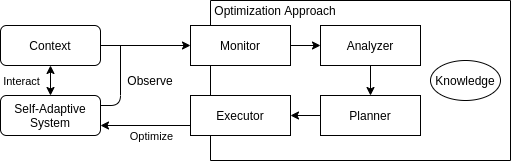
\includegraphics[width=0.8\textwidth]{images/ClassificationProposal-OptimizationMAPEK_horizontal.png}
    \caption{Mapping the optimization process to the \acrshort{mapek} feedback loop.}
    \label{fig:MappingOptMAPEK}
\end{figure}

This chapter will derive and propose a classification for \acrlong{oa}[es] for \acrlong{sas}
based on concepts that were discussed in chapter \ref{ch:SASClassification}.

\noindent Using the idea from Weyns et al. 2012 paper FORMS \cite*{FORMS} to compose \acrlong{sas}[s] from
layers of base and reflective components, 
an \acrlong{oa} for \acrlong{sas}[s] can be thought of
as a reflective component in a layer above the \acrshort{sas}. \\
This allows the application of multiple \acrshort{oa} to \acrshort{sas} and even the 
optimization of \acrshort{oa}. \\
It also establishes a connection between \acrshort{oa} and \acrlong{sas}[s].
This leads to the realization that a classification for \acrshort{oa} of \acrlong{sas}[s]
should be based upon the same principles as the classifications for \acrlong{sas}[s]. \\
Another benefit of this approach is a clear distinction between \acrlong{sas}[s] and \acrshort{oa} for \acrlong{sas}[s].
\acrlong{sas}[s] and \acrshort{oa} are both composed of reflective components and not base components. \\
Yet the Self-Adaptive System adapts base components, while the Optimization Approach adapts other reflective components.

\noindent Just like the adaptation process of \acrlong{sas}[s] can be understood using
the \acrshort{mapek} feedback loop by Kephart and Chess, 2003 \cite*{VisionOfAutonomicComputing}.
The process of optimizing a Self-Adaptive System can also be expressed using the \acrshort{mapek} feedback loop:
\begin{itemize}[nosep]
    \item Firstly the optimization approach has to constantly monitor the Self-Adaptive System and its context.
    \item The data gathered from monitoring can then be analyzed to decide wether or not an optimization is necessary and what should be optimized.
    \item After deciding that something should be optimized, there needs to be a plan on how to optimize.
    \item Lastly the planned optimization can be executed.
    \item During all of these steps the optimization approach requires knowledge about the Self-Adaptive System and its context.
\end{itemize}

\begin{figure}[h]
    \centering
    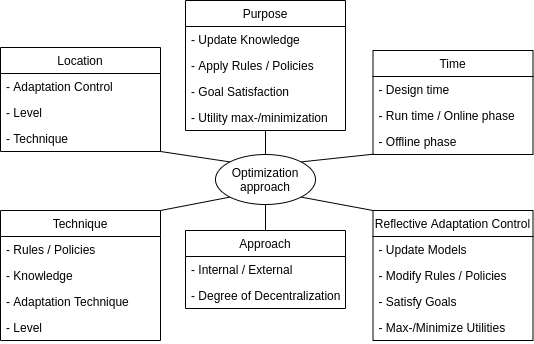
\includegraphics[width=0.8\textwidth]{images/ClassificationProposal-WithDimensions.png}
    \caption{The proposed classification for \acrlong{oa}[es] for \acrlong{sas}[s]}
    \label{fig:Proposal}
\end{figure}

\noindent Following Krupitzer's et al, 2015 \cite*{SurveyOnEngineeringApproaches} taxonomy for \acrlong{sas}[s],
a classification for Optimization Approaches of \acrlong{sas}[s] should answer 
the 5W+1H questions by Salehie and Tahvildari, 2009 \cite*{LandscapeAndResearchChallenges}.
These questions are: Where, When, What, Why, Who and How?

\noindent Figure \ref{fig:Proposal} shows the proposed classification for Optimization Approaches for \acrlong{sas}[s].
The classification consists of six dimensions: Location, Time, Purpose, Approach, Technique and Reflective Adaptation Control.
Each dimension is related to one of the 5W+1H questions.

\subparagraph*{Location}
Where in the system is an optimization necessary? \\
There are three main parts in a Self-Adaptive System that can be optimized as explained in chapter \ref{ch:SASClassification}.
These are:
\begin{itemize}[nosep]
    \item The Adaptation Control which can, for example, be optimized by changing or generating new adaptation rules.
    \item The Level on which adaptations are performed.
    \item The Technique that is used to perform adaptations.
\end{itemize}

\subparagraph*{Time}
When are optimizations performed? \\
Similarly to \acrlong{sas}[s], Optimization Approaches can be differentiated by comparing when they perform optimizations.
There are three different phases during the lifetime of a Self-Adaptive System where optimizations can occur.
These are:
\begin{itemize}[nosep]
    \item At the runtime of the system, which can also be called the online phase.
    \item During the design time of the system.
    \item While training the system or during its offline phase.
\end{itemize}
The training phase can happen in parallel to the run and design time of the system.
Examples for this would be when the initial parameters for a Self-Adaptive System are chosen by training a domain model
or when generating a new model for the system by training an updated domain model parallel to the running system.

\subparagraph*{Technique}
What gets changed to perform the optimization? \\
What gets changed in a Self-Adaptive System relates to where an optimization is necessary.
Thus, the following parts can be changed:
\begin{itemize}[nosep]
    \item The Rules / Policies used by the Adaptation Decision Criteria.
    \item The Knowledge of the system, which for example can consist of domain models.
    \item The Adaptation Technique used by the Self-Adaptive System.
    \item The Level on which the Self-Adaptive System performs changes.
\end{itemize}
One could argue that the Goals or especially Utility functions of a Self-Adaptive System could also be changed to optimize its performance.
In most cases this is not advisable because Goals and Utility functions can encode information
like legal or safety parameters, of which the system has no intrinsic knowledge.

\subparagraph*{Purpose}
Why should an optimization occur? \\
This is perhaps the most important question for any Optimization Approach as it determines if an optimization is necessary.
There can be several reasons for performing an optimization in a Self-Adaptive System:
\begin{itemize}[nosep]
    \item The system learned new information about, for example, its environment and needs to update its domain models.
    \item Due to external or internal changes, a Goal might not be satisfiable anymore.
    \item The difference of the actual versus the expected outcome of a rule / policy has exceeded a threshold.
    \item A Utility function needs to be maximized or minimized.
\end{itemize}

\subparagraph*{Approach}
Who is responsible for performing the optimization? \\
The original "Who?" question by Salehie and Tahvildari focuses on the level of human intervention that is need by the system.
\acrlong{sas}[s] have no need for human intervention, because they operate on clearly defined rule sets.
It is in the nature of Optimization Approaches for \acrlong{sas}[s] to change these rule sets.
This can lead to problems that make human intervention necessary.
A result of this is that, in contrast to the the taxonomy for \acrlong{sas}[s], 
the Approach for Optimization Approaches should have its own dimension.
\begin{itemize}[nosep]
    \item Is there an internal component that performs changes or are they performed by an external actor.
    \item Which degree of decentralization is used?
    Is each component responsible for itself (fully decentralized), are all components optimized by a central entity (fully centralized)
    or is a hybrid approach used?
\end{itemize}

\subparagraph*{Reflective Adaptation Control}
How is the optimization applied to the system? \\
Just like the Self-Adaptive System can be described by its Adaptation Control,
which is responsible for applying changes to the system,
an Optimization Approach can also be described by how it applies its optimizations to the system.
In reference to FORMS by Weyns et al., 2012\cite*{FORMS}, which uses reflective operations to change
components in the system, the Adaptation Control of the optimization approach will be called Reflective Adaptation Control.
The Reflective Adaptation Control can be classified by the following behaviors:
\begin{itemize}[nosep]
    \item Models: The system updates its models after receiving new information about its models.
    \item Rules / Policies: If the system detects, that it is in a state for which an adaptation rule/policy exists,
    it should perform that adaptation.
    \item Goals: Adaptation should be performed if the system does not meet pre-defined goals.
    \item Utility: An adaptation occurs to maximize or minimize a utility function.
\end{itemize}

\noindent Because the proposed classification is based upon the \acrshort{mapek} feedback loop and the 5W+1H questions,
it is useful to understand how they relate to each other.
This is depicted in Figures \ref{fig:MapeOA} and \ref{fig:QuestionsOA}.

\begin{figure}[h]
    \centering
    \begin{tabular}{|lcl|}
        \hline
        \acrlong{oa} & & \acrshort{mapek} \\
        \hline
        Location & & Monitor, Analyze, Execute \\
        \hline
        Time & & Monitor, Execute \\
        \hline
        Technique & & Plan, Execute \\
        \hline
        Purpose & & Analyze \\
        \hline
        Approach & & Plan, Execute \\
        \hline
        Reflective Adaptation Control & & Plan, Execute \\
        \hline
    \end{tabular}
    \caption{How the \acrshort{mapek} feedback loop by Kephart and Chess, 2003\cite*{VisionOfAutonomicComputing}
    relates to the dimensions of the classification for Optimization Approaches for \acrlong{sas}[s].}
    \label{fig:MapeOA}
\end{figure}

\begin{figure}[h]
    \centering
    \begin{tabular}{|lcl|}
        \hline
        \acrlong{oa} & & 5W+1H questions \\
        \hline
        Location & & Where \\
        \hline
        Time & & When \\
        \hline
        Technique & & What \\
        \hline
        Purpose & & Why \\
        \hline
        Approach & & Who \\
        \hline
        Reflective Adaptation Control & & How \\
        \hline
    \end{tabular}
    \caption{How the 5W+1H questions by Salehie and Tahvildari, 2009 \cite*{LandscapeAndResearchChallenges}
    relate to the dimensions of the classification for Optimization Approaches for \acrlong{sas}[s].}
    \label{fig:QuestionsOA}
\end{figure}

% TODO: Abschluss paragraph
\newpage
\section{Classifying Existing Optimization Approaches}
\label{ch:Existing}

% TODO:
% - Write a short explanation of each approach:
%     - FUSION
%     - Multi-Agent system
%     - Learning revised models
%     - Cloud performance and security
%     - FIoT
% - Classify each approach:
%     - FUSION
%     - Multi-Agent system
%     - Learning revised models
%     - Cloud performance and security
%     - FIoT

% \begin{itemize}
%     \item Classifying a selection of existing optimization approaches using the proposed classification.
% \end{itemize}

% \paragraph*{Literature for this section:} \begin{itemize}
%     \item "A multi-agent systems approach to autonomic computing" \cite{MultiAgentSystem}
%     \item "Using a multi-agent system and artificial intelligence for monitoring and improving the cloud performance and security" \cite{ImprovingCloudPerformanceAndSecurity}
% \end{itemize}

\subparagraph*{FUSION}
by Elkhodary et al, 2010 \cite*{FUSION}  uses a learning and an adaptation cycle.
The adaptation cycle corresponds to the Self-Adaptive part of the system
and does not directly affect the learning cycle.
The learning cycle is the optimization approach used by FUSION,
it changes the behavior of the adaptation cycle.
Both of these cycles continuously run in parallel to each other.
\begin{itemize}
    \item Location: FUSION optimizes the Adaptation Control.
    \item Time: FUSION uses both the design and run time to perform optimizations.
    The design time is used to generate an initial model for the learning cycle.
    During the run time the learning cycle monitors adaptations
    and updates the Knowledge Base to improve future adaptations.
    \item Technique: FUSION updates the rules used by the Self-Adaptive System and the shared knowledge base.
    \item Purpose: FUSION aims to decrease the difference between the expected and actual outcome of adaptation rules.
    \item Approach: FUSION acts as an external actor.
    \item Reflective Adaptation Control: FUSION applies optimizations by updating models and modifying rules.
\end{itemize}

\subparagraph*{Learning Revised Models for Planning in Adaptive Systems}
by Sykes et al., 2013 \cite*{LearningRevisedModels} uses
"a non-monotonic
probabilistic rule learning technique, NoMPRoL, that finds
hypotheses consisting of new rules specifying the probability
of an action achieving its specified outcome under particular
conditions" (Sykes et al., 2013 \cite*{LearningRevisedModels})
\begin{itemize}
    \item Location: The optimizations focus on the Adaptation Control.
    \item Time: The run time is used to perform optimizations.
    \item Technique: This approach optimizes the adaptation rules and domain models.
    \item Purpose: The optimizations aim to generate new and better adaptation rules and domain models.
    \item Approach: The optimizations are performed by an internal component that sits between the domain model
    and the Self-Adaptive System.
    \item Reflective Adaptation Control: This approach generates new adaptation rules.
\end{itemize}

\newpage
\subparagraph*{FIoT}
by Moraes do Nascimento and Pereira, 2016 \cite*{FIoT} is a framework for using agent-based systems
to construct self-organizing systems for the Internet of Things.
\begin{itemize}
    \item Location: FIoT optimizes three different levels: The physical, communication and application layer.
    \item Time: FIoT performs its optimizations during the run time of the system.
    \item Technique: FIoT changes the Level, Adaptation Technique and Rules / Policies of a Self-Adaptive System.
    \item Purpose: Generate self-organizing behavior in a Self-Adaptive System.
    \item Approach: FIoT uses a decentralized agent-based approach.
    \item Reflective Adaptation Control: 
\end{itemize}
\newpage
\section{Conclusion}
\label{ch:Conclusion}

\begin{itemize}
    \item Recommending future research directions: \begin{itemize}
        \item Applying the proposed classification to more existing optimization approaches.
        \item Possible directions for new optimization approaches.
    \end{itemize}
    \item What are the limitations of this paper?
\end{itemize}

%% --------------------
%% |   Bibliography   |
%% --------------------

%% Add entry to the table of contents for the bibliography
\printbibliography[heading=bibintoc]

\end{document}